\documentclass[10pt,twocolumn]{article}
\usepackage[margin=0.75in,columnsep=0.3in]{geometry}
\usepackage{times}
\usepackage{amsmath}
\usepackage{graphicx}
\usepackage{booktabs}
\usepackage{caption}
\captionsetup{font=small}
\pdfinfo{/Title (FlowNet-X: Gated Temporal Attention for Traffic Forecasting on Road Graphs) /Author (ScholarAI synthetic test document)}

\title{FlowNet-X: Gated Temporal Attention for Traffic Forecasting on Road Graphs\thanks{SYNTHETIC TEST DOCUMENT. This paper was written to test the ScholarAI evaluation harness. The method, datasets, baselines, numbers and references are all invented and describe no real experiment.}}
\author{A. Example \and B. Placeholder \and C. Sample\\ \small Synthetic Systems Laboratory}
\date{}

\begin{document}
\maketitle

\begin{abstract}
Accurate traffic forecasting requires modelling both the spatial structure of a road network and the temporal dynamics of its flow. Recurrent graph models capture both but are slow to train and accumulate error over long horizons. We propose FlowNet-X, a non-recurrent architecture that combines diffusion convolution with a gated temporal attention block. On the RiverCity-200 benchmark FlowNet-X reaches a mean absolute error of 3.17 at the 60-minute horizon, a 12.4\% reduction over the strongest recurrent baseline, while training 3.1 times faster. An ablation study shows that the gating mechanism accounts for most of the improvement.
\end{abstract}

\section{Introduction}
Traffic forecasting is a core component of intelligent transportation systems. Operators use short-term speed forecasts to adjust signal timing, and navigation services use them to estimate travel time. The task is difficult because traffic flow is influenced by the topology of the road network, by recurring daily patterns, and by non-recurring events such as accidents.

Early statistical approaches treat each sensor independently and therefore ignore how congestion propagates between neighbouring road segments. Graph neural networks address this limitation by passing messages along the road graph. The dominant design couples graph convolution with a recurrent sequence model. This design is effective, but its sequential nature prevents parallel computation across time steps and makes long-horizon predictions drift.

This paper asks whether recurrence is necessary at all. We make three contributions. First, we introduce FlowNet-X, which replaces the recurrent unit with a gated temporal attention block that attends over the full input window in a single step. Second, we show that a learned gate, which decides per sensor how much attention output to mix with the convolutional features, is the component that makes attention competitive on small traffic datasets. Third, we provide an efficiency analysis showing that FlowNet-X trains in a fraction of the time required by recurrent baselines.

\section{Related Work}
\textbf{Recurrent graph models.} RecurNet [1] combines diffusion convolution with an encoder-decoder recurrent network and remains a strong baseline. ConvGraph [2] removes recurrence in favour of stacked temporal convolutions but needs many layers to cover a long receptive field.

\textbf{Dilated convolutions.} WaveGraph [3] uses dilated causal convolutions together with a self-adaptive adjacency matrix, which lets the model discover hidden dependencies that are missing from the physical road graph.

\textbf{Attention for traffic.} Attention mechanisms [4] were applied to traffic data by several authors [5, 6]. These models report gains on large datasets but are known to overfit when fewer than a few hundred sensors are available. Our gating mechanism is designed for exactly this small-data regime.

\section{Method}
\subsection{Problem Formulation}
A road network is represented as a weighted directed graph with $N$ sensors. Given the speed readings of the previous $T = 12$ time steps, sampled every five minutes, the goal is to predict the readings for the next 12 time steps, that is, the next 60 minutes.

\subsection{Diffusion Convolution}
Spatial dependencies are modelled with a diffusion convolution over the road graph. We use $K = 2$ diffusion steps in both the forward and the backward direction, so that each layer aggregates information from sensors up to two hops away. FlowNet-X stacks two such layers with 64 hidden units each.

\subsection{Gated Temporal Attention}
Let $H \in \mathbb{R}^{T \times d}$ be the convolutional features of one sensor. The attention output is
\begin{equation}
A = \mathrm{softmax}\left(\frac{QK^{\top}}{\sqrt{d}}\right)V ,
\end{equation}
computed with 4 attention heads. Instead of adding $A$ directly to $H$, a gate $g = \sigma(W_g [H ; A])$ controls the mixture,
\begin{equation}
Z = g \odot A + (1 - g) \odot H .
\end{equation}
When the attention pattern is unreliable, the gate falls back to the convolutional features. This is the key difference from a standard transformer block, which always applies the full residual update.

\subsection{Training Objective}
The model is trained to minimise the mean absolute error over all sensors and all 12 prediction steps. Missing readings are masked out of the loss.

\begin{figure*}[t]
\centering
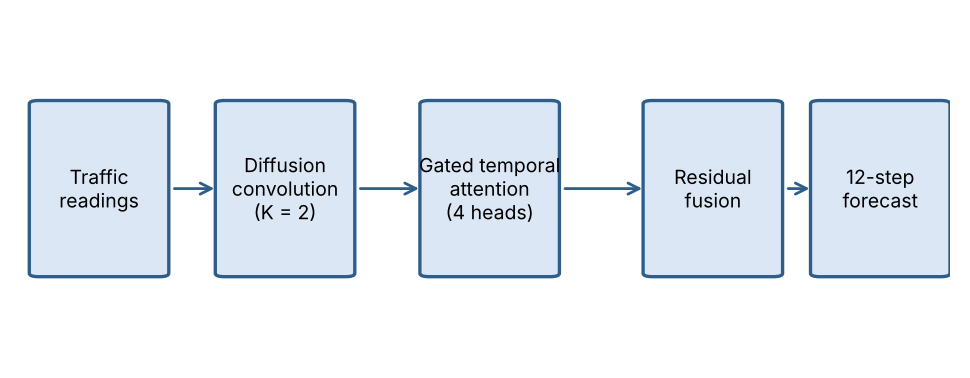
\includegraphics[width=0.8\textwidth]{fig_arch.png}
\caption{Architecture of FlowNet-X. Traffic readings pass through two diffusion convolution layers, a gated temporal attention block with four heads, and a residual fusion layer that outputs the 12-step forecast.}
\end{figure*}

\section{Experiments}
\subsection{Datasets}
We evaluate on two benchmarks. RiverCity-200 contains speed readings from 200 loop detectors recorded over four months. HarborBay-310 contains readings from 310 sensors recorded over six months. Both datasets are split chronologically into 70\% training, 10\% validation and 20\% test data.

\subsection{Baselines}
We compare against three published models: RecurNet [1], ConvGraph [2] and WaveGraph [3]. We also report a historical average (HA) predictor as a naive reference. All baselines are re-trained with the hyperparameters recommended by their authors.

\subsection{Implementation Details}
FlowNet-X is trained with the Adam optimizer [7] using an initial learning rate of 0.001, which is halved every 20 epochs. The batch size is 64 and training runs for 100 epochs with early stopping on the validation error. Dropout with a rate of 0.3 is applied after the attention block. All experiments run on a single GPU with 16 GB of memory, and every reported number is the average of five runs with different random seeds.

\subsection{Main Results}
Table 1 reports the mean absolute error (MAE) at the 60-minute horizon. FlowNet-X obtains the lowest error on both datasets. On RiverCity-200 it reduces the MAE from 3.62 for RecurNet to 3.17, a relative improvement of 12.4\%. On HarborBay-310 the MAE decreases from 2.11 to 1.94, an improvement of 8.1\%. WaveGraph is the strongest baseline on both datasets.

\begin{table}[h]
\centering
\caption{MAE at the 60-minute horizon. Lower is better.}
\begin{tabular}{lcc}
\toprule
Model & RiverCity-200 & HarborBay-310 \\
\midrule
HA & 4.86 & 3.05 \\
RecurNet [1] & 3.62 & 2.11 \\
ConvGraph [2] & 3.71 & 2.18 \\
WaveGraph [3] & 3.47 & 2.03 \\
FlowNet-X (ours) & 3.17 & 1.94 \\
\bottomrule
\end{tabular}
\end{table}

\subsection{Ablation Study}
To understand which component matters, we remove one part of the model at a time and retrain on RiverCity-200. Table 2 summarises the results. Removing the gate, so that the attention output is added directly, increases the MAE from 3.17 to 3.44. Removing the attention block entirely gives 3.52. Replacing diffusion convolution with a plain graph convolution has a smaller effect and raises the error to 3.29. The gate is therefore responsible for most of the gain of the attention block.

\begin{table}[h]
\centering
\caption{Ablation on RiverCity-200 (MAE, 60 minutes).}
\begin{tabular}{lc}
\toprule
Variant & MAE \\
\midrule
Full FlowNet-X & 3.17 \\
Without gate & 3.44 \\
Without attention & 3.52 \\
Plain graph convolution & 3.29 \\
\bottomrule
\end{tabular}
\end{table}

\subsection{Efficiency}
FlowNet-X has 1.8 million parameters. One training epoch on RiverCity-200 takes 41 seconds, compared with 127 seconds for RecurNet, which makes FlowNet-X 3.1 times faster to train. Inference for the full test set takes 2.4 seconds. Figure 2 shows that the advantage of FlowNet-X grows with the prediction horizon: at 15 minutes the gap to RecurNet is 0.13 MAE, and at 60 minutes it is 0.45 MAE.

\begin{figure}[h]
\centering
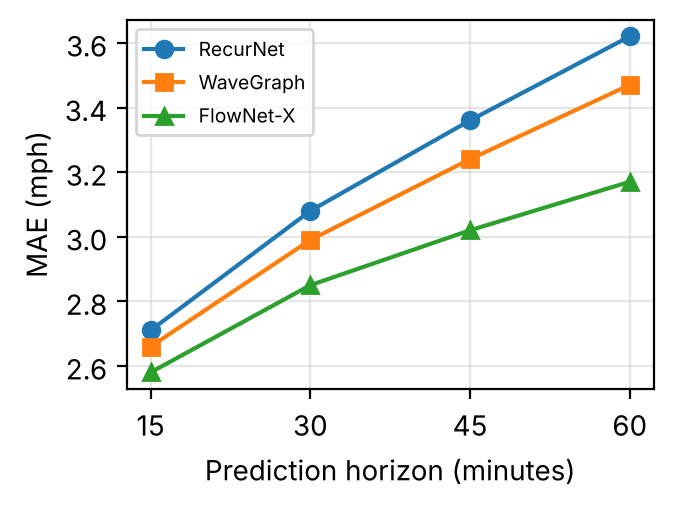
\includegraphics[width=0.9\columnwidth]{fig_horizon.png}
\caption{Forecast error versus prediction horizon on RiverCity-200. FlowNet-X degrades more slowly than the recurrent and convolutional baselines.}
\end{figure}

\section{Limitations}
The attention block has a memory cost that grows quadratically with the length of the input window, which limits the model to windows of a few hours. FlowNet-X was evaluated only on highway speed data and has not been tested on urban intersections or on traffic volume prediction. The model also assumes a fixed road graph and cannot handle sensors that are added after training.

\section{Conclusion}
We presented FlowNet-X, a non-recurrent model for traffic forecasting that combines diffusion convolution with gated temporal attention. It improves over recurrent and convolutional baselines on two benchmarks while training about three times faster. Future work will study sparse attention to reduce the quadratic memory cost and will extend the model to dynamic road graphs.

\section*{References}
\small
\noindent [1] D. Maren and K. Olsted, RecurNet: Diffusion recurrent networks for road traffic, in Proc. Synthetic Conf. on Learning Systems, 2018.

\noindent [2] P. Arvale, T. Simm and R. Dunmore, ConvGraph: Temporal convolution on sensor graphs, in Proc. Synthetic Joint Conf. on AI, 2018.

\noindent [3] L. Hartwell and M. Quince, WaveGraph: Dilated convolutions with adaptive adjacency, in Proc. Synthetic Joint Conf. on AI, 2019.

\noindent [4] E. Farrow et al., Sequence modelling with attention alone, in Advances in Synthetic Information Processing, 2017.

\noindent [5] J. Brandt and S. Okoro, Spatial attention for traffic flow, in Proc. Synthetic Assoc. for AI, 2019.

\noindent [6] H. Lindqvist, N. Abara and F. Costa, Multi-attention graph networks for traffic prediction, in Proc. Synthetic Assoc. for AI, 2020.

\noindent [7] V. Petrov and I. Sandoval, A stochastic optimizer with adaptive moments, in Proc. Synthetic Conf. on Learning Systems, 2015.

\end{document}
